\clearpage
\section{Tabellen \& Diverses}

\subsection{Grenzwerte}
\renewcommand*{\arraystretch}{2}
\begin{center}
	\begin{tabularx}{\linewidth}{XX}
		\toprule
		$\limxi \frac{e^x}{x^m} = \infty$                      & $\limxn xe^x = 0$                        \\
		$\limxi (1+x)^{\frac{1}{x}} = 1$                       & $\limxo (1+x)^{\frac{1}{x}} = e$         \\
		$\limxi (1+\frac{1}{x})^b = 1$                         & $\limxi n^{\frac{1}{n}} = 1$             \\
		$\limxo \frac{e^x-1}{x} = 1$                           & $\limxi (1-\frac{1}{x})^x = \frac{1}{e}$ \\
		$\lim_{x\to\pm\infty} (1 + \frac{k}{x})^{mx} = e^{km}$ & $\limxi (\frac{x}{x+k})^x = e^{-k}$      \\
		$\limxo \frac{\log 1 - x}{x} = -1$                     & $\limxo x \log x = 0$                    \\
		$\limxo \frac{e^{ax}-1}{x} = a$                        & $\limxo \frac{\ln(x+1)}{x} = 1$          \\
		$\lim_{x\to 1} \frac{\ln(x)}{x-1} = 1$                 & $\limxi \frac{\log(x)}{x^a} = 0$         \\
		\bottomrule
	\end{tabularx}
\end{center}

\begin{mainbox}{Partielle Integration}

	$$\int f'(x) g(x) \mathop{dx} = f(x)g(x) - \int f(x) g'(x) \mathop{dx}$$
\end{mainbox}
\begin{itemize}
	\item Meist gilt: Polynome ableiten ($g(x)$), wo das Integral periodisch ist ($\sin, \cos, e^x$,...) integrieren ($f'(x)$)
	\item Teils: mit $1$ multiplizieren, um partielle Integration anwenden zu können (z.B. im Fall von $\int \log(x) \mathop{dx}$)
\end{itemize}
\begin{mainbox}{Substitution}
	Um $\int_a^b f(g(x)) \mathop{dx}$ zu berechnen: Ersetze $g(x)$ durch $u$ und integriere $\int_{g(a)}^{g(b)} f(u) \frac{\text{d}u}{g'(x)}$.
\end{mainbox}
\begin{itemize}
	\item $g'(x)$ muss sich herauskürzen, sonst nutzlos.
	\item Grenzen substituieren nicht vergessen.
	\item Alternativ: unbestimmtes Integral berechnet werden und dann $u$ wieder durch $x$ substituieren.
	\item Man kann auch das Theorem in die andere Richtung anwenden: \[\int_a^b f(u) \mathop{du} = \int_{g^{-1}(a)}^{g^{-1}(b)}f(g(x))g'(x) \dx\]
	\item Sei $\X, Y$ kompakt, $f: Y \subset \R^n \to \R$ stetig.

	      Sei $\gamma: \X \to Y$ mit $\X = \X_0 \cup B, Y = Y_0 \cup C$ ($B, C$ Rand von $\X, Y$).

	      Wenn $\gamma: \X_0 \to Y_0$ bijektiv und $C^1$ mit det$(J_\gamma(x)) \neq 0, \forall x \in \X_0$, dann gilt
	      \[\int_Y f(y)\mathop{dy} = \int_{\X} f(\gamma(x))|\text{det}(J_\gamma(x))|\dx\]
\end{itemize}

\subsection{Ableitungen}
\begin{center}
	% the c>{\centering\arraybackslash}X is a workaround to have a column fill up all space and still be centered
	\begin{tabularx}{\linewidth}{c>{\centering\arraybackslash}Xc}
		\toprule
		$\mathbf{F(x)}$                        & $\mathbf{f(x)}$          & $\mathbf{f'(x)}$         \\
		\midrule
		$\frac{x^{-a+1}}{-a+1}$                & $\frac{1}{x^a}$          & $\frac{a}{x^{a+1}}$      \\
		$\frac{x^{a+1}}{a+1}$                  & $x^a \ (a \ne 1)$        & $a \cdot x^{a-1}$        \\
		$\frac{1}{k \ln(a)}a^{kx}$             & $a^{kx}$                 & $ka^{kx} \ln(a)$         \\
		$\ln |x|$                              & $\frac{1}{x}$            & $-\frac{1}{x^2}$         \\
		$\frac{2}{3}x^{3/2}$                   & $\sqrt{x}$               & $\frac{1}{2\sqrt{x}}$    \\
		$-\cos(x)$                             & $\sin(x)$                & $\cos(x)$                \\
		$\sin(x)$                              & $\cos(x)$                & $-\sin(x)$               \\
		$\frac{1}{2}(x-\frac{1}{2}\sin(2x))$   & $\sin^2(x)$              & $2 \sin(x)\cos(x)$       \\
		$\frac{1}{2}(x + \frac{1}{2}\sin(2x))$ & $\cos^2(x)$              & $-2\sin(x)\cos(x)$       \\
		\multirow{2}*{$-\ln|\cos(x)|$}         & \multirow{2}*{$\tan(x)$} & $\frac{1}{\cos^2(x)}$    \\
		                                       &                          & $1 + \tan^2(x)$          \\
		$\cosh(x)$                             & $\sinh(x)$               & $\cosh(x)$               \\
		$\log(\cosh(x))$                       & $\tanh(x)$               & $\frac{1}{\cosh^2(x)}$   \\
		$\ln | \sin(x)|$                       & $\cot(x)$                & $-\frac{1}{\sin^2(x)}$   \\
		$\frac{1}{c} \cdot e^{cx}$             & $e^{cx}$                 & $c \cdot e^{cx}$         \\
		$x(\ln |x| - 1)$                       & $\ln |x|$                & $\frac{1}{x}$            \\
		$\frac{1}{2}(\ln(x))^2$                & $\frac{\ln(x)}{x}$       & $\frac{1 - \ln(x)}{x^2}$ \\
		$\frac{x}{\ln(a)} (\ln|x| -1)$         & $\log_a |x|$             & $\frac{1}{\ln(a)x}$      \\
		\bottomrule
	\end{tabularx}
\end{center}
\subsection{Weitere Ableitungen}
\begin{center}
	\begin{tabularx}{\linewidth}{>{\centering\arraybackslash}X>{\centering\arraybackslash}X}
		\toprule
		$\mathbf{F(x)}$ & $\mathbf{f(x)}$             \\
		\midrule
		$\arcsin(x)$    & $\frac{1}{\sqrt{1 - x^2}}$  \\
		$\arccos(x)$    & $\frac{-1}{\sqrt{1 - x^2}}$ \\
		$\arctan(x)$    & $\frac{1}{1 + x^2}$         \\
		$x^x \ (x > 0)$ & $x^x \cdot (1 + \ln x)$     \\
		\bottomrule
	\end{tabularx}
\end{center}
% \subsection{Integrale}
% \begin{center}
% 	\begin{tabularx}{\linewidth}{>{\centering\arraybackslash}X>{\centering\arraybackslash}X}
% 		\toprule
% 		$\mathbf{f(x)}$                              & $\mathbf{F(x)}$                                                  \\
% 		\midrule
% 		$\int f'(x) f(x) \mathop{dx}$                & $\frac{1}{2}(f(x))^2$                                            \\
% 		$\int \frac{f'(x)}{f(x)} \mathop{dx}$        & $\ln|f(x)|$                                                      \\
% 		$\int_{-\infty}^\infty e^{-x^2} \mathop{dx}$ & $\sqrt{\pi}$                                                     \\
% 		$\int (ax+b)^n \mathop{dx}$                  & $\frac{1}{a(n+1)}(ax+b)^{n+1}$                                   \\
% 		$\int x(ax+b)^n \mathop{dx}$                 & $\frac{(ax+b)^{n+2}}{(n+2)a^2} - \frac{b(ax+b)^{n+1}}{(n+1)a^2}$ \\
% 		$\int (ax^p+b)^n x^{p-1} \mathop{dx}$        & $\frac{(ax^p+b)^{n+1}}{ap(n+1)}$                                 \\
% 		$\int (ax^p + b)^{-1} x^{p-1} \mathop{dx}$   & $\frac{1}{ap} \ln |ax^p + b|$                                    \\
% 		$\int \frac{ax+b}{cx+d} \mathop{dx}$         & $\frac{ax}{c} - \frac{ad-bc}{c^2} \ln |cx +d|$                   \\
% 		$\int \frac{1}{x^2+a^2} \mathop{dx}$         & $\frac{1}{a} \arctan \frac{x}{a}$                                \\
% 		$\int \frac{1}{x^2 - a^2} \mathop{dx}$       & $\frac{1}{2a} \ln\left| \frac{x-a}{x+a} \right|$                 \\
% 		$\int \sqrt{a^2+x^2} \mathop{dx} $           & $\frac{x}{2}f(x) + \frac{a^2}{2}\ln(x+f(x))$                     \\
% 		\bottomrule
% 	\end{tabularx}
% \end{center}
\begin{subbox}{Gamma-Verteilung}
	Die Gamma-Verteilung ist eine stetige Verteilung mit der Dichtefunktion
	\[f(z) = \frac{1}{\Gamma(\alpha)}\lambda^{\alpha}z^{\alpha-1}e^{-\lambda z} \text{ für } z \geq 0, \alpha >0, \lambda > 0\]
	\begin{enumerate}
		\item Wir schreiben $Z \sim Ga(\alpha, \lambda)$ für eine gamma-verteilte Zufallsvariable $Z$ mit Parametern $\alpha$ und $\lambda$.
		\item Die Summe von $n \in \N$ unabhängigen $Exp(\lambda)$-verteilten Zufallsvariablen ist $Ga(n, \lambda)$-verteilt.
		\item Die $\chi^2$-Verteilung mit $k$ Freiheitsgraden ist $Ga\left(\frac{k}{2}, \frac{1}{2}\right)$-verteilt.
	\end{enumerate}
\end{subbox}
Sei $(X_i)_{i \geq 1} \sim \mathcal{N}(0,1)$ iid. eine Folge von Zufallsvariablen.
\begin{enumerate}
	\item $\sum_{i = 1}^{n} X_i^2 \sim \chi^2_n$
	\item $\frac{1}{n}(\sum_{i = 1}^n X_i)^2 \sim \chi_1^2$
	\item $X_1^2 + X_2^2 \sim Exp\left(\frac{1}{2}\right)$
	\item Sei $Y \sim \chi_m^2$ unabhängig von $X \sim \mathcal{N}(0,1)$. Dann gilt \[\frac{X}{\sqrt{\frac{1}{m}Y}} \sim t_m\]
	\item Es gilt $\lim_{m\to\infty} t_m \sim \mathcal{N}(0,1)$ verteilt, für endliche $m$ is $t_m$ langschwänziger als $\mathcal{N}(0,1).$
\end{enumerate}
Seien $X_1, \ldots, X_n$ iid. $\sim \mathcal{N}(\mu, \sigma^2)$.
Wir erinneren uns an die Notationen für Stichprobenmittel $\overline{X}_n$ und Stichprobenvarianz $S^2 = \frac{1}{n-1}\sum_{i = 1}^n(X_i - \overline{X}_n)^2$.
\begin{enumerate}
	\item $\frac{n-1}{\sigma^2}S^2 \sim \chi_{n-1}^2$
	\item $\overline{X}_n$ und $S^2$ sind unabhängig.
	\item \[\frac{\overline{X}_n - \mu}{S/\sqrt{n}} = \frac{\frac{\overline{X}_n - \mu}{\sigma / \sqrt{n}}}{\sqrt{S^2/\sigma^2}} \sim t_{n-1}\]
\end{enumerate}

\subsection{MLE Schätzer}
\begin{itemize}
	\item $X_1, ..., X_n \sim Exp(\theta)$ iid.: $T = \frac{n}{\sum_{i=1}^n X_i} = \frac{1}{\overline{X}_n}$
	\item $X_1, ..., X_n \sim Geo(\theta)$ iid.: $T = \frac{n}{\sum_{i=1}^n X_i} = \frac{1}{\overline{X}_n}$
	\item $X_1, ..., X_n \sim Bin(N, \theta)$ iid.: $T = \frac{1}{N}\frac{\sum_{i = 1}^n X_i}{n}$
	\item $X_1, ..., X_n \sim P(\theta)$ iid.: $T = \frac{\sum_{i = 1}^n X_i}{n} = \overline{X}_n$
	\item $X_1, ..., X_n \sim \mathcal{U}([\theta_1, \theta_2])$ iid.: $T_{\theta_1} = \min(X_i), T_{\theta_2} = \max(X_i)$
	\item $X_1, ..., X_n \sim \mathcal{N}(\theta_1, \theta_2)$ iid. : $T_{\theta_1} = \overline{X}_n, \ T_{\theta_2} = S^2$
\end{itemize}

\clearpage
\section{Diskrete Verteilungen}

\renewcommand{\arraystretch}{5}
\resizebox{.99\linewidth}{!}{
	\setlength\tabcolsep{1.5pt}
	\centering
	\begin{tabular}{||c|p{3.3cm}|*{4}{c|}|}
		\hline
		Verteilung                                                   & Parameter                                                                & $\mathbb{E}[X]$                     & Var($X$)                          & $p_X(t)$                     & $F_X(t)$                 \\
		\hline
		Gleichverteilung                                             & $n$: Anzahl Ereignisse \newline $x_i$: Ereignisse                        & $\frac{1}{n}\sum_{i=1}^{n}x_i$      & $\frac{1}{n}\sum_{i=1}^{n}x_i^2 -
		\frac{1}{n^2}\left(\sum_{i=1}^n x_i \right)^2$               & $\frac{1}{n}$                                                            & $\frac{|\{k:x_k \leq
		t\}|}{n}$                                                                                                                                                                                                                                                                   \\
		\hline

		Bernoulli                                                    & $p$: ErfolgsWK                                                           & $p$                                 & $p \cdot (1-p) $                  & $p^t(1-p)^{1-t}$             & $1-p$ für $0 \leq t < 1$ \\
		\hline

		Binomial                                                     & $p$: ErfolgsWK\newline$n$: Anzahl Versuche                               & $np$                                & $np(1-p)$                         & $\binom{n}{t}p^t(1-p)^{n-t}$ &
		$\sum_{k=0}^t\binom{n}{k}p^k(1-p)^{n-k}$                                                                                                                                                                                                                                    \\
		\hline

		Geometrisch                                                  & $p$: ErfolgsWK\newline$t$: Anzahl Versuche                               & $\frac{1}{p}$                       & $\frac{1-p}{p^2}$                 &
		$p(1-p)^{t-1}$                                               & $1-(1-p)^t$                                                                                                                                                                                                  \\
		\hline

		Negativ Binomial                                             & $r>0$: Erfolge bis Abbruch\newline$p$: ErfolgsWK\newline$t$: Misserfolge &
		$\frac{pr}{1-p}$                                             & $\frac{pr}{(1-p)^2}$                                                     & $\binom{t+r-1}{k} \cdot (1-p)^rp^t$ &
		$F_{\text{Binomial}}(t;n=t+r,p)$                                                                                                                                                                                                                                            \\
		\hline

		Hypergeometrisch                                             & $N$: Anzahl aller Elemente\newline$M \leq N$: Anzahl möglicher
		Erfolge\newline$n \leq N$: Anzahl Elemente in der Stichprobe & $n\frac{M}{N}$                                                           &
		$n\frac{M}{N}\left(1-\frac{M}{N}\right)\frac{N-m}{N-1}$
		                                                             & \raisebox{-5pt}{$\frac{\binom{M}{t}\binom{N-M}{n-t}}{\binom{N}{n}}$}     &
		\raisebox{-5pt}{$\sum_{k=0}^{t}\frac{\binom{M}{k}\binom{N-M}{n-k}}{\binom{N}{n}}$}                                                                                                                                                                                          \\
		\hline

		Poisson                                                      & $\lambda$: Erwartungswert und Varianz                                    & $\lambda$                           & $\lambda$                         &
		$\frac{\lambda^k}{k!}e^{-\lambda}$                           & $p$                                                                                                                                                                                                          \\
		\hline
	\end{tabular}}
\section{Stetige Verteilungen}

\resizebox{.99\linewidth}{!}{
	\setlength\tabcolsep{1.5pt}
	\centering
	\begin{tabular}{||c|p{2cm}|*{4}{c|}|}
		\hline
		Verteilung                                                                                     & Parameter                                                                          & $\mathbb{E}[X]$            & Var($X$)                                                                             & $f_X(t)$ & $F_X(t)$ \\
		\hline

		Gleichverteilung                                                                               & $[a,b]$: Intervall                                                                 & $\frac{a+b}{2}$            & $\frac{1}{12}(b-a)^2$                                                                &
		$\frac{1}{b-a}$                                                                                & $\frac{t-a}{b-a}$                                                                                                                                                                                                            \\
		\hline

		Exponentialverteilung                                                                          & $\lambda: \frac{1}{\mathbb{E}[X]}$                                                 & $\frac{1}{\lambda}$        &
		$\frac{1}{\lambda^2}$                                                                          & $\begin{cases} \lambda e^{-\lambda t}&t\geq 0\\0&t<0\end{cases}$                   &
		$\begin{cases}1-e^{-\lambda t}&t>0\\0&t\leq 0\end{cases}$                                                                                                                                                                                                                                                                     \\
		\hline

		Normalverteilung                                                                               & $\sigma^2$: Varianz \newline $\mu: \mathbb{E}[X]$                                  & $\mu$                      & $\sigma^2$                                                                           &
		\raisebox{-5pt}{$\frac {1}{\sqrt {2\pi \sigma^{2}}}e^{-{\frac {(t-\mu )^{2}}{2\sigma ^{2}}}}
		-\infty <t<\infty $}                                                                           & \raisebox{-5pt}{${\frac {1}{\sigma {\sqrt {2\pi }}}}\int _{-\infty }^{t}e^{-{\frac
		{1}{2}}\left({\frac {y-\mu }{\sigma }}\right)^{2}}\mathrm {d} y$}                                                                                                                                                                                                                                                             \\
		\hline

		$\chi^2$-Verteilung                                                                            & $m$: Freiheitsgrad                                                                 & $m$                        & $2m$                                                                                 & $\frac
			{1}{2^{\frac {m}{2}}\Gamma ({\tfrac {m}{2}})}t^{{\frac {m}{2}}-1}e^
		{-{\frac {t}{2}}}\quad t>0$                                                                    & Gamma$(\frac{m}{2}, \frac{t}{2})$                                                                                                                                                                                            \\[8pt]
		\hline

		Gamma-Verteilung                                                                               & $\alpha,\lambda$                                                                   & $\frac{\alpha}{\lambda}$   & $\frac{\alpha}{\lambda^2}$                                                           &
		\raisebox{-5pt}{${\begin{aligned}{\frac {\lambda ^{\alpha }t^{\alpha -1}e^{-\lambda t}}{\Gamma
							                  (\alpha )}}\quad t>0\quad \alpha ,\lambda >0\end{aligned}}$} & ${\frac
		{1}{\Gamma (\alpha )}}\gamma (\alpha ,\lambda t)$                                                                                                                                                                                                                                                                             \\[10pt]
		\hline

		t-Verteilung                                                                                   & $n$: Freiheitsgrad                                                                 & $0$ für $n>1$ sonst undef. & $\begin{cases} \frac{n}{n-2} &
              n > 2           \\ \infty & 1 < n \leq 2 \\ \text{undef.} & \text{sonst}\end{cases}$ &
		\raisebox{-2pt}{$\frac{\Gamma\left( \frac{n+1}{2}\right)}{\sqrt{n\pi} \cdot \Gamma(\frac{n}{2})}
		\left(1 + \frac{t^2}{n}\right)^{- \frac{n+1}{2}}$}                                             & oof                                                                                                                                                                                                                          \\[10pt]
		\hline

		Chauchy-Verteilung                                                                             & $x_0$: Lageparameter \newline $\gamma$: Skalenparameter                            & undef.                     & undef.                                                                               &
		$\frac{1}{\pi\gamma\left[1+\left(\frac{t-x_0}{\gamma}\right)^2\right]}$                        & $\frac{1}{2} + \frac{1}{\pi} \arctan\left(\frac{t-x_0}{\gamma}\right)$                                                                                                                                                       \\
		\hline
	\end{tabular}}

\renewcommand{\arraystretch}{1}

\vspace*{0.2cm}
\begin{subbox}{Gamma-Funktion}
	\begin{align*}
		\Gamma(v) := \int_0^\infty t^{v-1}e^{-t}\mathop{dt}, v \geq 0.
	\end{align*}
	Es gilt $\Gamma(n) = (n-1)!$ für $n \in \N$.
\end{subbox}
\begin{subbox}{Binomischer Lehrsatz}
	\[(x + y)^n = \sum_{k = 0}^n  \binom{n}{k} x^{n-k}y^k\]
\end{subbox}
\begin{subbox}{Cauchy Produkt}
	Falls $\sum_{n= 0}^\infty a_n$ und $\sum_{n = 0}^\infty b_n$ absolut konvergent, dann folgt
	\[\sum_{n = 0}^\infty \sum_{k = 0}^n a_kb_{n-k} = \sum_{n = 0}^\infty \sum_{i+j = n} a_ib_j = \left(\sum_{n = 0}^\infty a_n\right) \cdot \left(\sum_{k = 0}^\infty b_k\right)\]
\end{subbox}

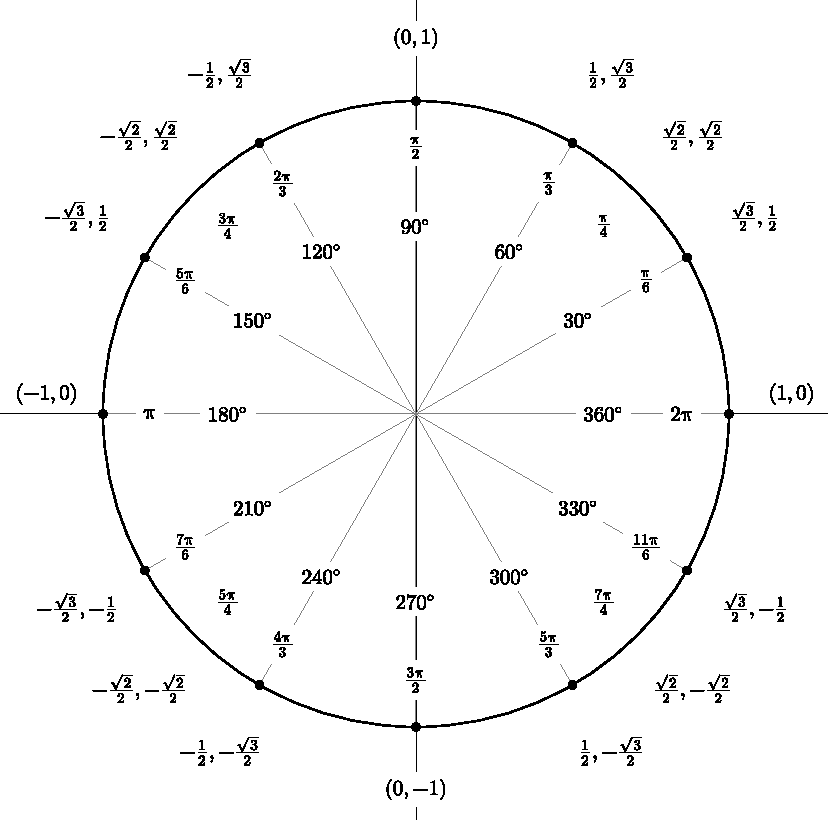
\includegraphics[width=\linewidth]{degrees_circle.pdf}

\begin{subbox}{$\chi^2$-Verteilung}
	Sind die Zufallsvariablen $X_1, ..., X_n$ i.i.d. $\sim \mathcal{N}(0,1)$, dann ist
	\[\sum_{i = 1}^n X_i^2 \sim \chi^2_m\]

	\begin{itemize}
		\item $\chi^2_m$ ist eine Gamma-Verteilung mit $\alpha = \frac{m}{2}$ und $\lambda = \frac{1}{2}$.
		\item Falls $m = 2$, dann ist $\chi^2_2$ eine Exponentialverteilung mit $\lambda = \frac{1}{2}$.
	\end{itemize}
\end{subbox}

\begin{subbox}{t-Verteilung}
	Seien $X \sim \mathcal{N}(0,1)$ und $Y \sim \chi^2_m$ unabhängig. Dann ist
	\[T = \frac{X}{\sqrt{\frac{Y}{m}}} \sim t_m\]

	\begin{itemize}
		\item $t_m$ ist symmetrisch um $0$.
		\item Für $m = 1$ ist $t_1$ Cauchy-verteilt.
		\item $t_n$ ist langschwänziger als $\mathcal{N}(0,1)$.
		\item $\lim_{m\to\infty} t_m = \mathcal{N}(0,1)$.
	\end{itemize}
\end{subbox}
